\documentclass[a4paper,12pt]{report}
\usepackage[utf8]{inputenc}
\usepackage{graphicx}
\usepackage[margin=1in]{geometry}
\usepackage{setspace}
\usepackage{amsmath}
\usepackage{caption}
\usepackage{subcaption}
\usepackage{hyperref}

%\usepackage{titlesec}
\usepackage{listings}
\begin{document}
\chapter{Installing and Running OpenFOAM and ParaView}
\section{Introduction to OpenFOAM}
\flushleft OpenFOAM, which stands for Open source
 Field Operation And Manipulation, is a free and open source CFD toolbox. It is a C++ library / toolkit,
used primarily to create executables, known as applications. These applications fall into
 two major categories:
 \begin{itemize}
   \item \textbf{Solvers} – designed to solve a specific problem in continuum mechanics
   \item \textbf{Utilities} - designed to perform tasks that involve data manipulation
 \end{itemize}
 \flushleft OpenFOAM has a vast range of solvers spanning from complex fluid flows involving chemical reactions, turbulence and heat transfer, to solid dynamics and electromagnetics. These numerical solvers cover both 2-Dimensional and 3-Dimensional problems. A comprehensive structure of OpenFOAM can be given as \ref{1}:
 
\begin{figure}[ht]  
\begin{center}  
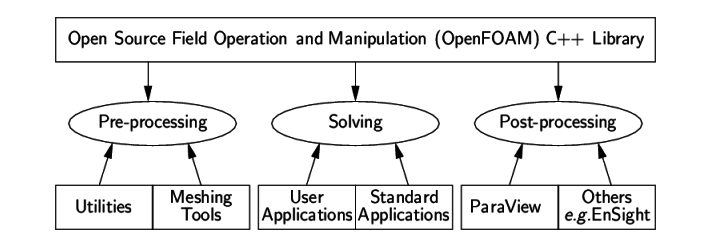
\includegraphics[scale=0.5]{1.png}
\caption{Overall structure of OpenFOAM}
\label{1}
\end{center}  
\end{figure}

\flushleft Nowadays, OpenFOAM is extensively used in academia
 and industry to solve wide variety of computational problems. The parallelization capability of OpenFOAM for both pre and post-processing of data provides the users with an efficient environment for working.  One of the major advantage of using OpenFOAM is that in contrast to any proprietary software, this source code here is accessible and modifiable.
 \section{Introduction to ParaView}
 \flushleft ParaView is a multi-platform, open-source software used for data analysis and scientific visualization application.It is built based on Visualization Tool-Kit (VTK) libraries. It uses qualitative and quantitative techniques to built the visualization. ParaView was largely developed to analyze huge data sets using distributed memory computing resources. It analyzes data interactively both in 3-Dimension as well as programmatically using it's batch processing capabilities. 
 \flushleft It is a user-friendly data visualization software which utilizes Cmake for its compilation.Paraview is predominantly used for post-processing in OpenFOAM due to its unique ability to run on distributed and shared memory, parallel and single processor systems.
 \flushleft OpenFOAM and Paraview can be very easily installed in your systems by mainly following the user manual for installation.There are many ways of installing OpenFOAM and ParaView in your systems. Here we will be discussing two basic ways of installation in a LINUX environment.
 
 \section{Installation of OpenFOAM and ParaView through Synaptic Package Manager}
 \flushleft Here in this section we will discuss how to install OpenFOAM-2.4.0 and ParaView-4.1.0 using Synaptic Package Manager. To understand this chapter our readers should have a prior exposer to LINUX based operating systems along with its basic commands and also some trivial knowledge on Computational Fluid Dyanmics (CFD). 
 \flushleft In a LINUX operating system, on theleft side of your computer screen you can see the Launcher with the list of softwares.
 \flushleft To install OpenFOAM and ParaView, click on the search box as shown in figure \ref{2} on top of the Launcher and type Synaptic. This will display the Synaptic Package Manager. Click on it to open.
 
\begin{figure}[h]  
\begin{center}  

\includegraphics[scale=0.8]{2.png}
\caption{Search Icon on top of Launcher}
\label{2}
\end{center}  
\end{figure}
 
 \flushleft Here you would be interrupted with the system authentication. After poviding the system password press enter.
 \vspace{5cm}
 \begin{figure}[h]  
\begin{center}  
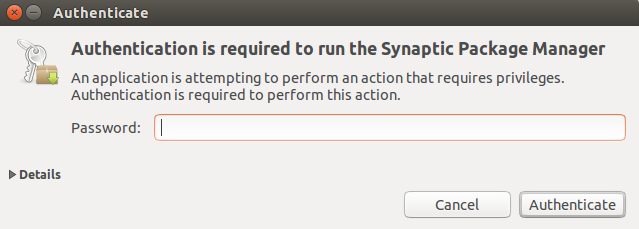
\includegraphics[scale=0.4]{3.png}
\caption{Enter the system password here}
\end{center}  
\end{figure}


\flushleft Once the Synaptic Package Manager is Opened, in the search box (as shown in figure \ref{4} ) type OpenFOAM.

\begin{figure}[ht]  
\begin{center}  
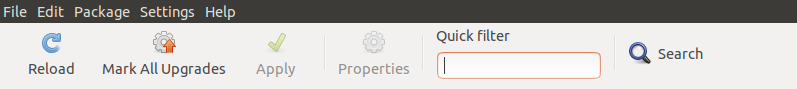
\includegraphics[scale=0.4]{4.png}
\caption{Type OpenFOAM in the search box}
\label{4}
\end{center}  
\end{figure}

\flushleft You will see both OpenFOAM-2.3.0 and Paraview-4.1.0, as shown in figure \ref{5}. Right click on both of them for installation and click Apply to install. It will take a while for installation depending upon your internet speed.

\begin{figure}[ht]  
\begin{center}  
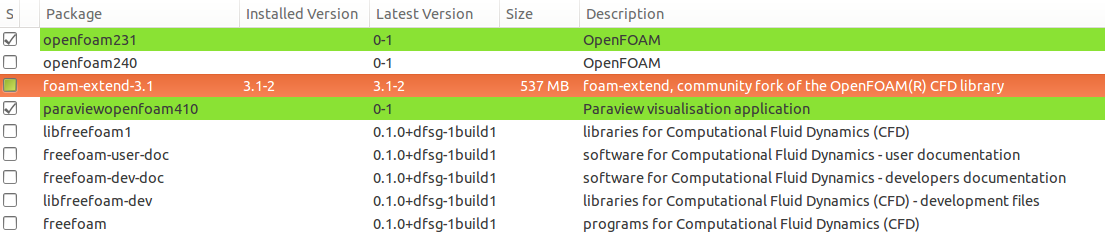
\includegraphics[scale=0.33]{5.png}
\caption{Click on OpenFOAM and Paraview to Mark and Install}
\label{5}
\end{center}  
\end{figure}

\section{Installation of OpenFOAM and ParaView through OpenFOAM Website}
\flushleft OpenFOAM can also be downloaded and installed through the OpenFOAM website by carrying out the following steps:
\begin{enumerate}
  \item On your browser type \url{www.openfoam.com/download}
  \item Go to Ubuntu Debian Installation
  \item Open the terminal window by pressing Ctl+Alt+t keys simultaneously on your keyboard or you can also open it using the search icon on top of the Launch bar
  \item Under the first point of Installation copy the command line from the website and paste it in your terminal window

\begin{figure}[ht]  
\begin{center}  
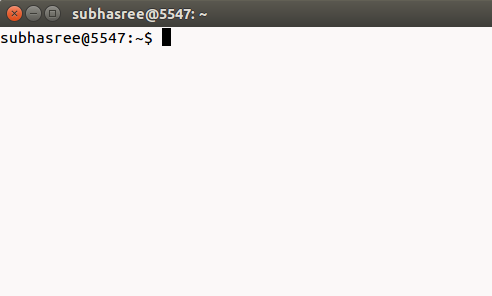
\includegraphics[scale=0.5]{6.png}
\caption{Press Ctrl+Alt+t keys to open up terminal window}
\label{terminal}
\end{center}  
\end{figure}

 \item For complete installation for OpenFOAM and Paraview follow the steps under installation
 \end{enumerate}
 
 \section{Configure OpenFOAM and ParaView}
 \flushleft To configure the installed software we need to source this application by editing the bashrc file. To do this, open a new command terminal and type:
\begin{lstlisting}[frame=single]
gedit ~/.bashrc
\end{lstlisting}

\flushleft and press enter.

\begin{figure}[ht]  
\begin{center}  
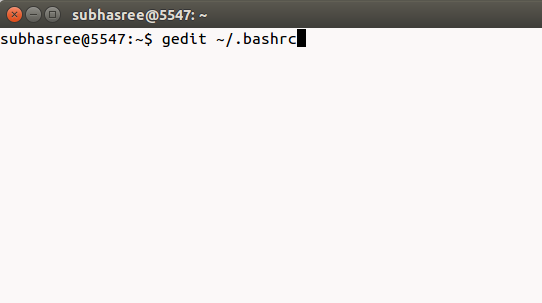
\includegraphics[scale=0.4]{7.png}
\caption{Open the bashrc file}
\label{7}
\end{center}  
\end{figure}

\flushleft After the bashrc file is opened scroll down to the bottom of the file. Then go back to your browser (OpenFOAM download page) and scroll down to User Configuration.
\flushleft Copy the second command line
\begin{lstlisting}[frame=single]
source /opt/openfoam230/etc/bashrc 
\end{lstlisting}
\flushleft under this heading and paste it at the bottom of the bashrc file. Save it and close the file.

\section{Test the Installed Software}
\flushleft To check whether OpenFOAM is installed properly open a new command terminal and  type icoFoam -help and press enter. You will see a ”Usage” message on your terminal screen, as shown in figure \ref{8}. This shows that the installation is done.

\begin{figure}[ht]  
\begin{center}  
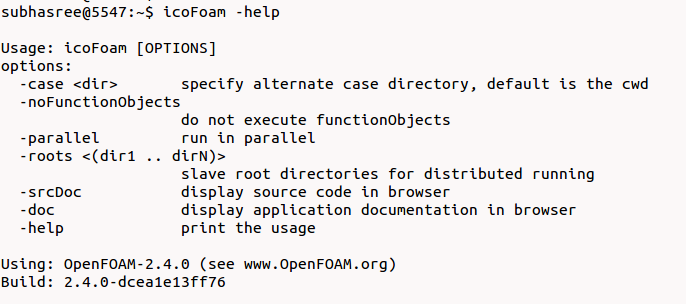
\includegraphics[scale=0.5]{8.png}
\caption{Usame message}
\label{8}
\end{center}  
\end{figure}

\flushleft You may also install OpenFOAM and Paraview by compiling the Source code available under the header of Source Pack Installation on the OpenFOAM website. Download the tar files. Create a folder in your Home directory by the name OpenFOAM and paste the tar files in that folder. Extract the files in that folder.
\flushleft Follow the steps given on the OpenFOAM source pack installation page to complete the installation. Since we compile the source code it might take a few hours to complete.

\section{Creating User Working Directory}
\flushleft Before proceeding further with an example case file, we will first discuss how to create a working directory for the users.
\flushleft Follow the steps given below:
\begin{enumerate}
\item Open up a new terminal and type the following and press enter
  \begin{lstlisting}[frame=single]
  mkdir -p $FOAM_RUN
  \end{lstlisting}
\item After this type
  \begin{lstlisting}[frame=single]
  cp -r $FOAM_TUTORIALS $FOAM_RUN
  \end{lstlisting}
\end{enumerate}
\flushleft This will copy the tutorials folder into the user's directory.

\section{Running OpenFOAM and ParaView}
\flushleft Here in this section we will teach how to run openFOAM and ParaView using an example \textbf{Lid Driven Cavity} case file. This case file is already written in the OpenFOAM tutorial folder. 
\flushleft This example is a two dimensional problem where the upper plate moves at a mentioned user defined speed while the other three sides of the plate are stationary as shown in figure \ref{9}. The solver we use here is icoFoam which is an Transient solver for incompressible flow.

\begin{figure}[ht]  
\begin{center}  
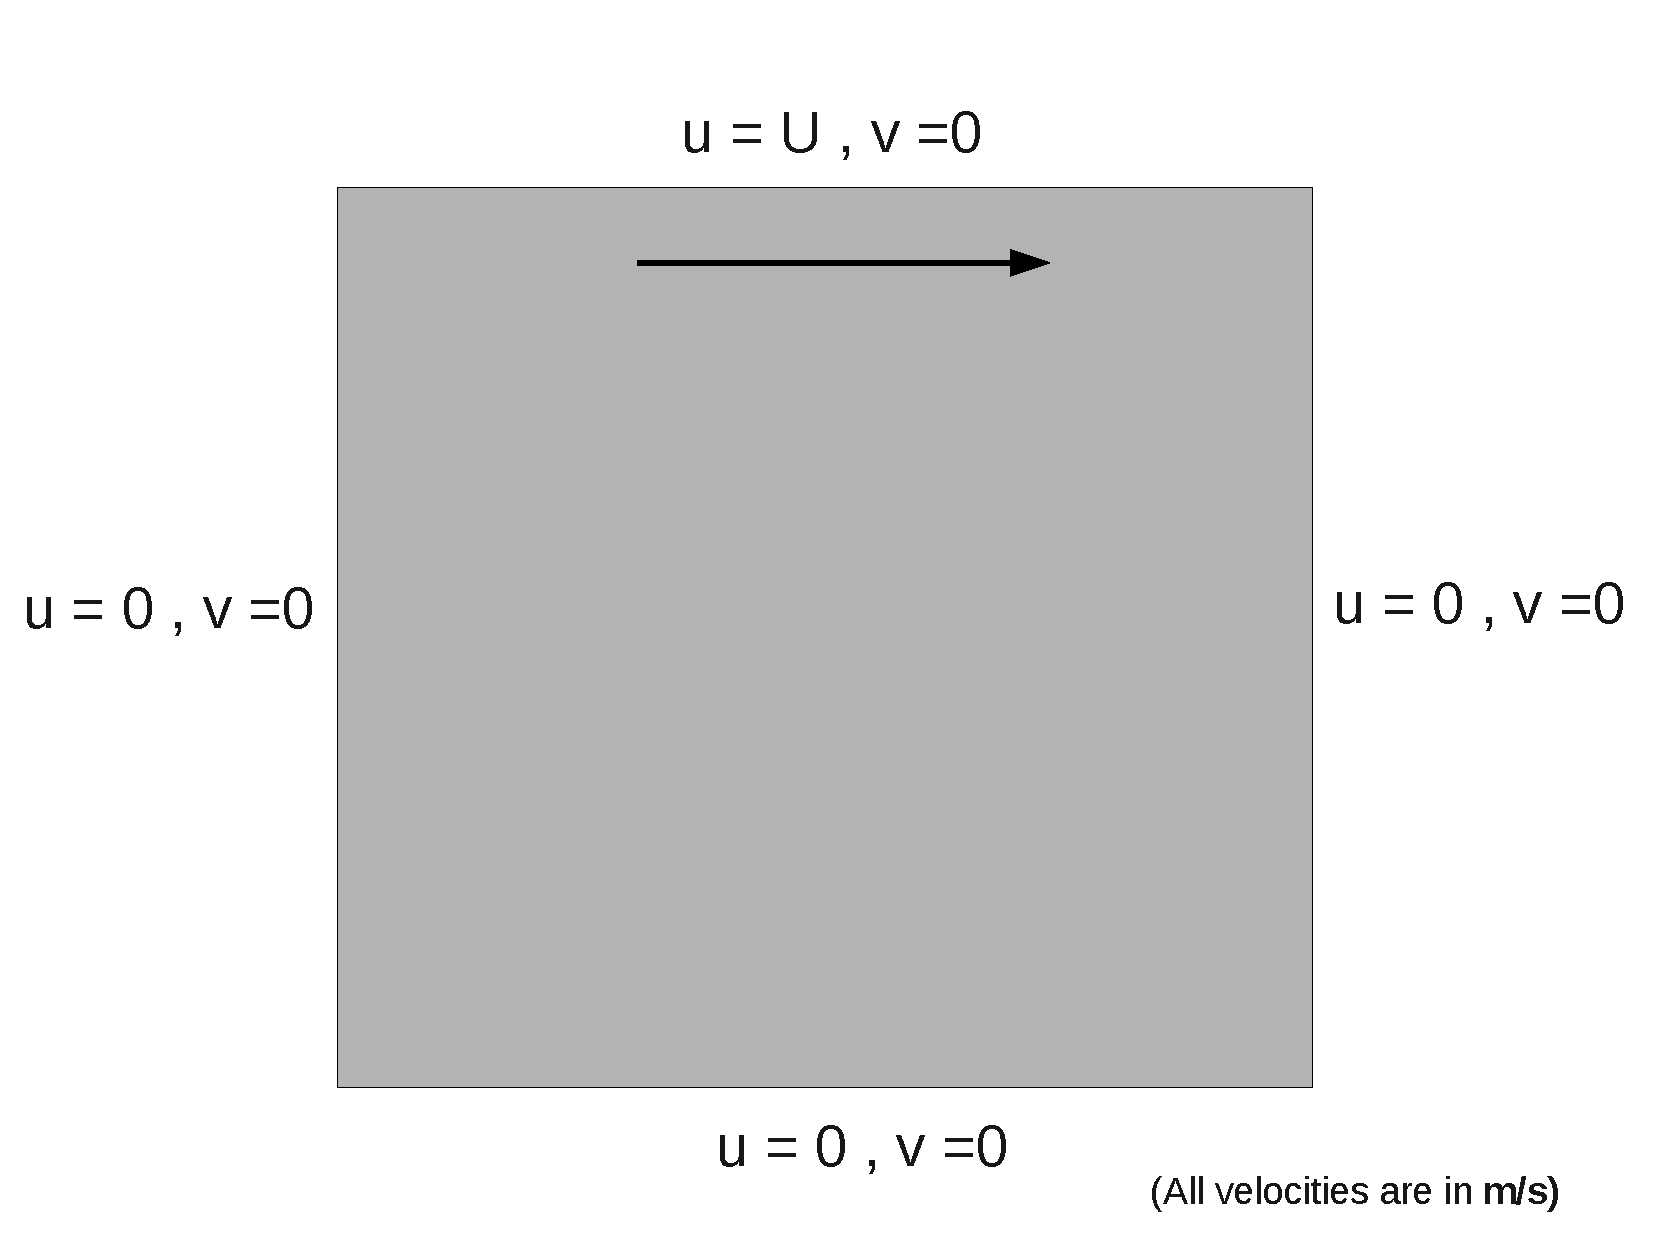
\includegraphics[scale=0.3]{9.pdf}
\caption{Example problem solved after OpenFOAM installation}
\label{9}
\end{center}  
\end{figure}

In the terminal copy paste the path given below :

\begin{lstlisting}[frame=single]
cd OpenFOAM/OpenFOAM-2.3.0/run/tutorials/incompressible/icoFoam
/cavity
\end{lstlisting}
  
\flushleft The geometry now needs to be meshed. This can be done using the blockMesh utility of OpenFOAM. In the command terminal type blockMesh and press enter which completes the meshing and you will see the following details as shown in figure \ref{10}

  \begin{figure}[ht]  
\begin{center}  
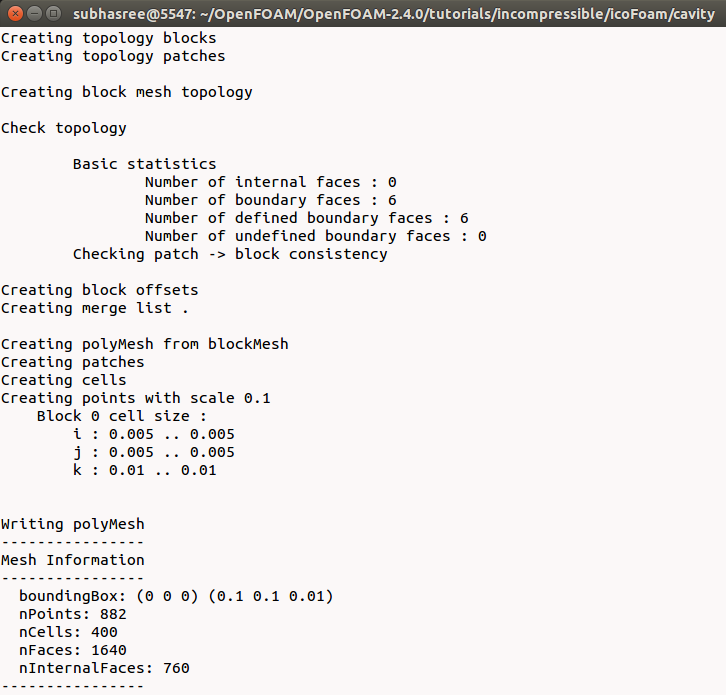
\includegraphics[scale=0.3]{10.png}
\caption{BlockMesh utility for Meshing in OpenFOAM}
\label{10}
\end{center}  
\end{figure}
\vspace{10cm}
\flushleft Once meshing is done we will now run the solver by typing icoFoam in the command terminal. The iteration running can be seen in the terminal window, as shown in figure \ref{11}. Thus in this section we have learned how to solve a problem case in OpenFOAM. 

\begin{figure}[ht]  
\begin{center}  
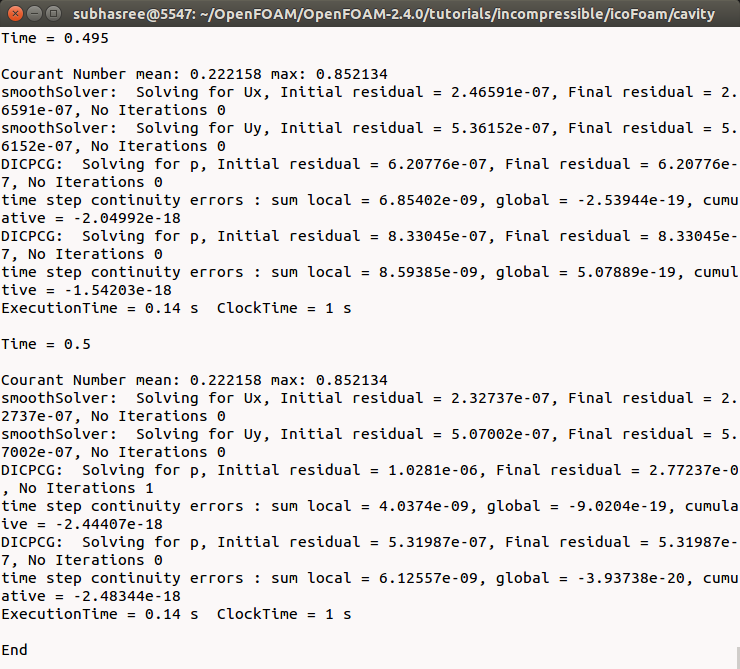
\includegraphics[scale=0.3]{11.png}
\caption{Terminal shows the iterations running}
\label{11}
\end{center}  
\end{figure}
\flushleft Now we will learn how to post-process this data. The solution can be Visualized using Paraview. To open ParaView window type \textbf{paraFoam} in your terminal and press enter. This will open up the paraview window, as shown in Figure \ref{12}.
\vspace{5cm}
\begin{figure}[ht]  
\begin{center}  
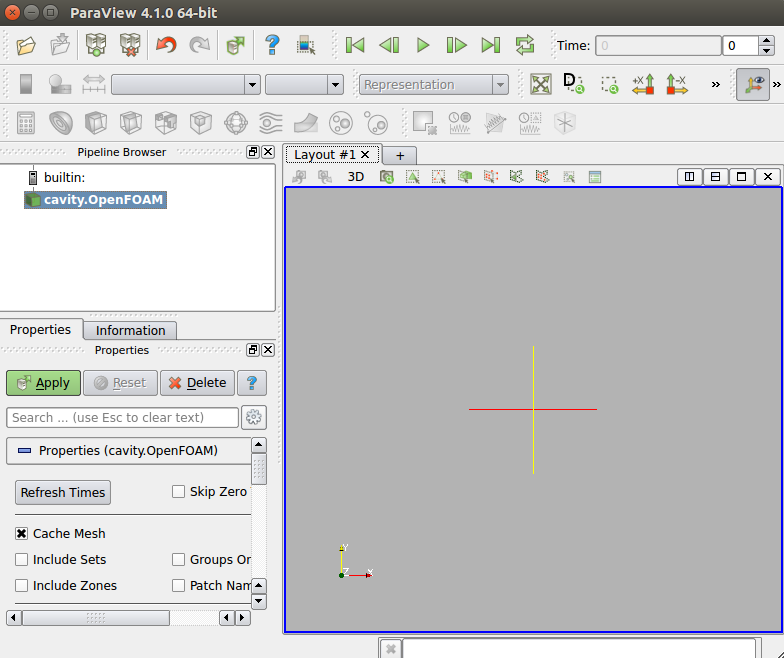
\includegraphics[scale=0.32]{12.png}
\caption{Paraview window}
\label{12}
\end{center}  
\end{figure}
\flushleft Click on the Apply button on the left hand side of the Object Inspector Menu to view the Geometry, as shown in figure \ref{13}.

\begin{figure}[ht]  
\begin{center}  
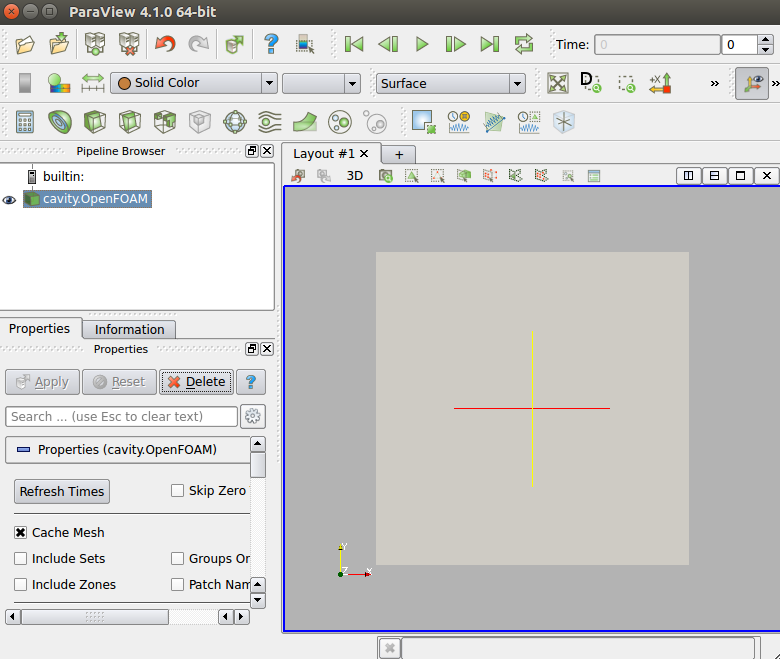
\includegraphics[scale=0.32]{13.png}
\caption{Geometry seen in the Paraview Window}
\label{13}
\end{center}  
\end{figure}

\flushleft To check the Boundary conditions scroll down the object inspector menu and go down to mesh parts and uncheck internal mesh option and click apply. You will see that the geometry disappears, as shown in figure \ref{14}.
\vspace{15cm}
\begin{figure}[ht]  
\begin{center}  
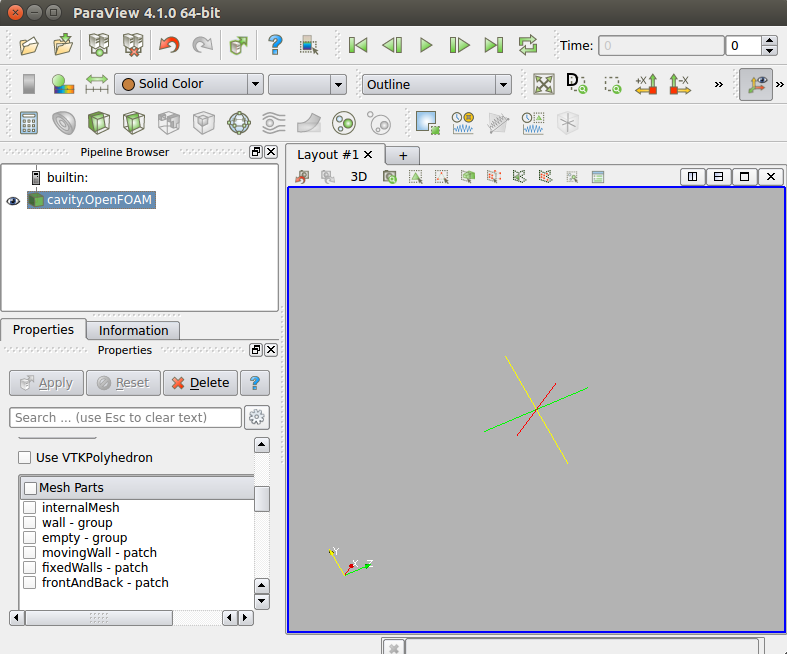
\includegraphics[scale=0.32]{14.png}
\caption{Uncheck the internal mesh option}
\label{14}
\end{center}  
\end{figure}

\flushleft Now click on the checkbox for movingWall and fixedWall and click the apply button. You can see the moving wall and fixedWall in the paraview window, as shown in figure \ref{15}. You can also uncheck the movingWall option to see the fixedWalls in the paraview window,as shown in Figure \ref{16}.

\begin{figure}[ht]  
\begin{center}  
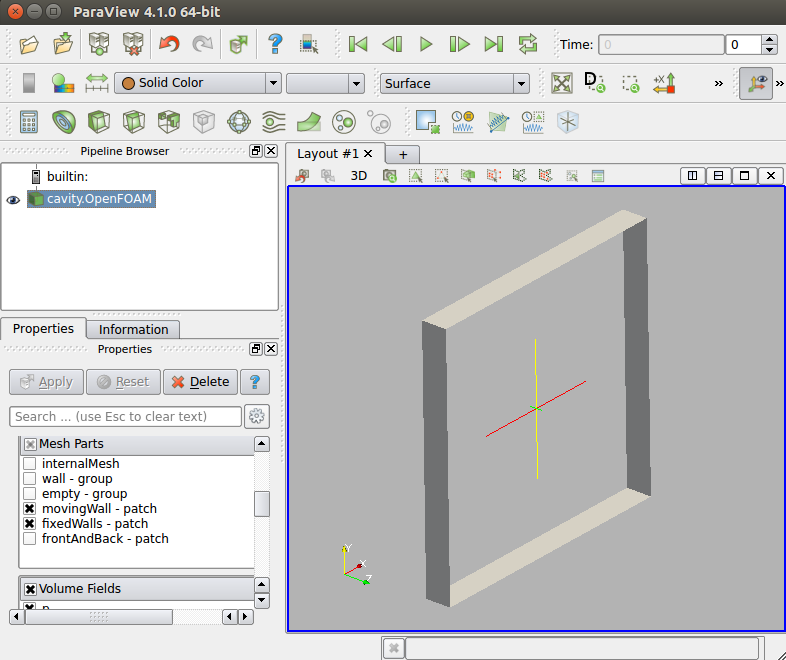
\includegraphics[scale=0.32]{15.png}
\caption{Check for the moving and fixedWalls in paraview window}
\label{15}
\end{center}  
\end{figure}

\begin{figure}[ht]  
\begin{center}  
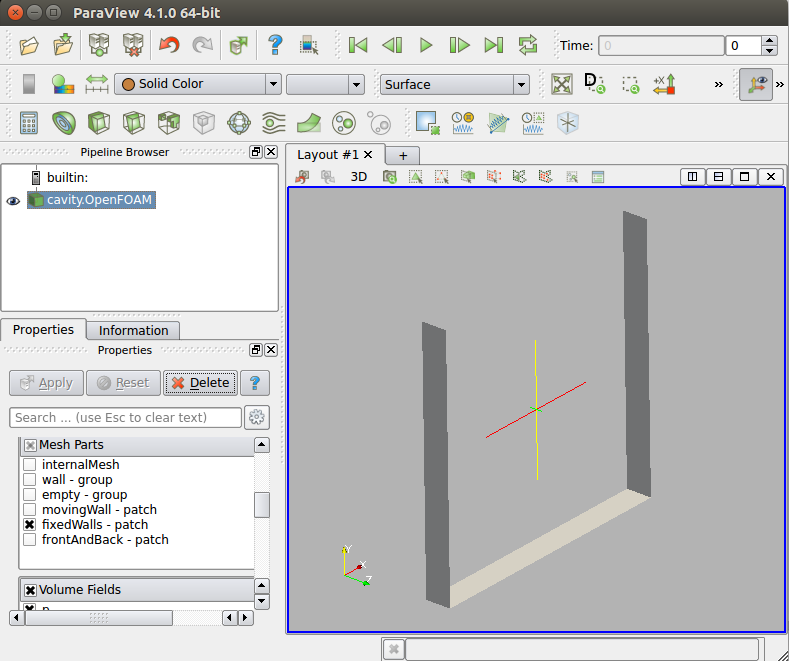
\includegraphics[scale=0.32]{16.png}
\caption{FixedWalls appear in the paraview window}
\end{center}  
\end{figure}

\end{document}
